\chapter{Finetuning method to increase quality of document
embeddings}\label{chapter:training_method}

In this chapter we describe our method of training document embeddings. Our
approach is based on teacher-student training approach, where we distil the
knowledge of two teacher embedding models into a single student model. In
Section~\ref{section:training_method} we explain our training method in detail
and roughly define the used loss function. Then in
Section~\ref{section:teacher_models} we describe the two teacher models, which
we use in the rest of the thesis. Finally, in
Sections~\ref{section:structural_loss}~and~\ref{section:contextual_loss} we
walk through each of the two loss components in detail.

\section{Training methodology}\label{section:training_method}

% \begin{itemize}
%     \item what is teacher-student training
%     \item our approach to training is to use teacher-student training
%     \item motivation to do so -- reference document representation chapter
%     \item two teachers -- structural and contextual teacher
% \end{itemize}

Our training methodology aims to train an embedding model such that its
embeddings more faithfully represent the input. As we described in
Chapter~\ref{chapter:document_representation} we distinguish two qualities of
faithful representations: structural and contextual. The goal is to instill
both of these two qualities into a single embedding model. To do so, we use
teacher-student training with two teacher text embedding models, one with high
structural capacity, the other with high contextual capacity.

In the following subsections we describe teacher-student training in detail and
give high-level overview of the proposed loss function.

\subsection{Teacher-student training}

In teacher-student training we train a single \emph{student} model based on a
non-trainable \emph{teacher} model. The goal is to make the student model to
imitate the teacher model and thereby digest the teacher's understanding of the
input. Teacher-student training is useful in a number of situations. For
instance it used to overcome some inherit limitation of the teacher model such
as its large size~\citep{sanh2019distilbert}. Also, teacher-student training
can be used to enforce some kind of alignment between models'
outputs~\citep{reimers2020making}. The motivation to align the model's outputs
often comes from an intuition about language, such as that embeddings of
two translations of a given sentence should be the close to each other.

In our setting, we assume two embedding models $\Teacher_S$, $\Teacher_C$ with
high structural and contextual capacities respectively. Teacher-student
training allows us to instill both of these capacities into a third model
{\Student}, while also avoiding some of the architectural limitations of both
reference models. For convenience we call $\Teacher_S$ \emph{structural
teacher}, $\Teacher_C$ \emph{contextual teacher}, and {\Student}
\emph{student}.


\subsection{Abstract loss formulation}

% \begin{itemize}
%     \item there are two losses corresponding to the two reference models
%     \item weighting the two training losses -- structural model will not be applicable
%         for long inputs
% \end{itemize}

Our loss function should align the output of a student model {\Student} with
outputs of two teacher models $\Teacher_S$, and $\Teacher_C$. We use two
similarity functions $\Loss_S$, $\Loss_C$ that compare the student's embedding
$y_\Student$ with structural teacher embedding $y_{\Teacher_S}$ and with
contextual teacher embedding $y_{\Teacher_C}$ respectively. As we are unsure
which balance of $\Loss_S$ and $\Loss_C$ is optimal we introduce weighting
parameter $\lambda$ that balances the effect of the two losses on the final
loss. In the most general form, we can assume $\lambda$ to be dependent on the
input text $x$, since the performance of the teacher models might vary across
different inputs. In particular, we can expect $\lambda$ to be dependent on the
length of the input, since for shorter inputs the context is minimal and
therefore expendable. The form of the loss as we have described it is defined
in Equation~\ref{eq:abstract_loss}. We explore concrete options for $\Loss_S$,
$\Loss_C$ and $\lambda(x)$ in Chapter~\ref{chapter:experiments}.

\begin{equation}\label{eq:abstract_loss}
  \Loss(
    x,
    y_\Student,
    y_{\Teacher_S},
    y_{\Teacher_C},
    \lambda
  ) =
    \lambda(x) \Loss_S(y_\Student, y_{\Teacher_S}) +
            \Loss_C(y_\Student, y_{\Teacher_S})
\end{equation}

\section{Teacher models}\label{section:teacher_models}

% \begin{itemize}
%     \item what models we used as teachers
%     \item why we chose as we did
% \end{itemize}

In this section we present the teacher models we use during our experiments in
Chapter~\ref{chapter:experiments}. We highlight why we choose the particular
models and how we obtain the their embeddings. We chose
Sentence-BERT~\citep{reimers2020making} (or \emph{SBERT}) as the structural
teacher model, and Paragraph Vector~\citep{le2014distributed} (or \emph{PV}) as
the context teacher model.

\subsection{SBERT}

Sentence-BERT~\citep{reimers2019sentence} is a composition of a
BERT-like~\citep{devlin2019bert} encoder with a mean pooling layer above its
final hidden states. We have chosen SBERT as structural teacher for its
Transformer architecture, which as we have discussed in
Chapter~\ref{chapter:document_representation}, has high structural capacity.
Additionally, SBERT is finetuned on NLI datasets to increase its text
understanding and to produce embeddings which are semantically meaningful.

There are several versions of SBERT, that differ in the base Transformer
encoder, from which is SBERT warm-started and then finetuned. We use SBERT
warm-started from MPNet~\citep{song2020mpnet}, that achieves high scores across
many sentence embedding
benchmarks\footnote{\url{https://sbert.net/docs/pretrained_models.html}}, while
being reasonably small. To be exact we use its Hugging Face implementation
named \\ \texttt{sentence-transformers/all-mpnet-base-v2}.

We generate the embeddings of any training dataset directly without any
additional finetuning.

\subsection{Paragraph Vector}

Paragraph Vector~\cite{le2014distributed} (also known as Doc2Vec) is a simple
text-embedding model that views the input as a Bag of Words (or BoW). Paragraph
Vector is composed of two sub-models called Distributed Memory (DM) and
Distributed Bag of Words (DBOW). In practice one or both models can be used,
where the final embedding is the concatenation of all sub-models' outputs. Both
models construct embedding of the whole input with which they predict a
randomly masked out input word. DM additionally uses embeddings of neighbouring
words.

We choose Paragraph Vector as contextual teacher due to its unique architecture
that forces the model to develop a single vector, that summarizes the common
theme of the document. Moreover, Paragraph Vector does not have limited maximum
input length, and so as a contextual teacher it will always provide some signal
to the student regarding the document's context. Also, even though Paragraph
Vector cannot match the performance of a substantially more complex models such
as Transformers, \cite{dai2015document} show that for larger datasets Paragraph
Vector outperforms classical embedding models such as Latent Dirichlet
Allocation~\citep{blei2003latent} or TF-IDF weighted BoW
model~\citep{harris1954distributional}.

We generate Paragraph Vector's embeddings after training the model on
\emph{all} training datasets for which we require a contextual teacher's
embedding. There are many hyperparameters that govern how Paragraph Vector is
trained. Since there are no universally agreed best-performing values for any
of them, we see these as hyperparameters of our teacher-student training
method. We explore the effect of some of these parameters on the model's
performance in Chapter~\ref{chapter:experiments}.

TODO: my own graphic here

\begin{figure}[h]
    \centering
    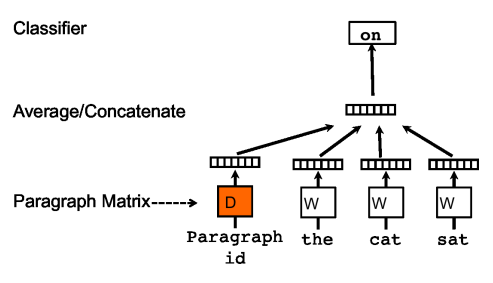
\includegraphics[width=0.4\textwidth]{./img/pv-dm.png}
    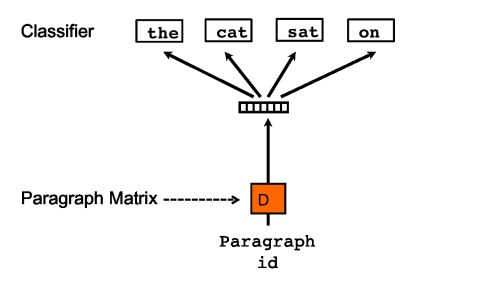
\includegraphics[width=0.4\textwidth]{./img/pv-dbow.png}
    \caption{PV-DM and PV-DBOW architectures.\label{fig:pv-dm_pv-dbow}}
\end{figure}
